\chapter{\label{ch:6-eval}Evaluation}

\minitoc

In this chapter, we evaluate our proposed approach. We start by describing a method for randomly generating benchmark operation graphs. Then, we present the obtained results. Finally, we give the speedup and accuracy results obtained by applying our approach on an industrial use case.

\section{Random Generator of Dependence Graphs}

Due to the difficulty in acquiring enough industrial FMU co-simulation applications for assessing our approach, we had to use a random generator of FMU dependence graphs. The generator creates the graphs and characterizes them with attributes.

\subsection{Random Dependence Graph Generation}

The random generator that we have implemented is inspired by random generator presented in \cite{kalla:2004}. However, it differs from this work in that the generation is done in two stages. In other words, we have to generate, first, the different FMUs of the co-simulation and their internal structures. Second, we generate the dependence graph by creating inter-FMU dependence in such a way that the resulting operation graph is a DAG. The proposed generator is based on a technique of assignment of operations to levels. The level of an operation is the number of operations on the longest path from a source operation to this operation. The dependence graph can then be visualized on a grid of levels as depicted in figure \ref{}. 


The generator uses the following parameters:

\begin{itemize}
\item The graph size $n$: the number of operations;
\item The number of FMUs $m$;
\item The graph height $h$: the number of levels in the graph
\item The graph width $w$: the maximum number of nodes on one level
\end{itemize}

Note that parameters $n$ and $m$ are related. In other words, for a given size of a graph $n$, an adequate number of FMUs $m$ has to be chosen. 

The generation of the dependence graph is performed as follows:
\begin{itemize}
\item \textbf{Input:} Size of the graph $n$, number of FMUs $m$, height of the graph $h$, and width of the graph $w$. %The number of FMUs can be derived automatically from the size of the graph using a predefined formula. For instance, one of the formulas that we have used is $ m = 5 \times log10(n/5)$. This allows to have adequate size of the graph and number of FMUs. Suppose, for example, that we have a size $n = 1000$ and a number of FMUs $m = 1$. Obviously, this example does not represent a realistic application. 
\item \textbf{Step 1:} Randomly distribute the $n$ operations across the $m$ FMUs. Given the number of operations of each FMU, we randomly determine the number of its input operations and the number of its output operations. Every FMU has one state operation.
\item \textbf{Step 2:} Randomly generate the intra-FMU arcs. This step is controlled by two parameters.  The number of arcs to generate and the number of NDF outputs of the FMU. These outputs are not considered when randomly generating the arcs.
\item \textbf{Step 3:} Randomly assign the operations to the grid levels. This step is performed by assigning output operations and then input operations repeatedly.
\begin{enumerate}
\item Assign all NDF operations to level $0$ of the grid.
\item Randomly assign remaining output operations to even levels $lvl \in {2, 4, \ldots, h-3} $ of the grid.
\item Assign the input operations to the odd levels $lvl \in {1, 3, \ldots, h-4} $ of the grid such that any input operation $o_i$ that is connected to an output operations $o_j$ (intra-FMU dependence) is assigned to the level preceding the level to which $o_j$ has been assigned. 
\item Assign the remaining input operations (each of which is not connected with any output operation) to the level $h-2$ of the grid. These operations will be connected only with the state operations of their respective FMUs.
\item Add the state operations to the last level of the grid.
\end{enumerate}
\item \textbf{Step 4:} Create the arcs of the dependence graph. At this step we randomly generate inter-FMU dependence. For each operation $o_i$ on the level $lvl$ of grid, we randomly select an output operation $o_j$ from the preceding level $lvl-1$ and which belongs to a different FMU than $o_i$. We create an arc from $o_j$ to $o_i$. If no such output operation is found at level $lvl-1$, we select randomly an output operation from any level $lvl' < lvl-1$ and connect it with the operation $o_i$. Finally the arcs from input and output operations to state operations are created. 
\end{itemize}

\subsection{Random Dependence Graph Characterization}

In addition to random generation of the dependence graph structure, we need to generate the attributes of the graph. In particular, the following attributes are generated by our random generator:
\begin{itemize}
\item Communication steps of the FMUs.
\item Execution times of the operations. The execution times are generated randomly in such a way that state operations have longer execution times than the output and input operations
\end{itemize}

\section{Results}

We have carried out different tests in order to evaluate our proposed approach. For both the acyclic orientation and the scheduling, we compared the execution time of our proposed heuristic with the execution time of the ILP, and the objective result of the heuristic with the objective result of the ILP. For ILP resolution, we used three solvers: lpsolve, Gurobi, and CPLEX. With lpsolve, we were only able to solve small instances of the scheduling problem. Gurobi was more efficient but we obtained the best performance using CPLEX. Therefore, the results presented hereafter were obtained using CPLEX. %Tests have been carried out on different multi-core PCs. In the following, we indicate, when necessary, the characteristics of the platform used.  
Tests were performed on a desktop computer with a 6-core Intel Xeon processor running at 2.7 GH and 16GB RAM.

\subsection{Execution Time of the Acyclic Orientation Algorithms}

In order to compare the execution time of our acyclic orientation heuristic with the execution time of the acyclic orientation ILP, we have generated 85 random operation graphs of different sizes between five and $10000$. %First we generated the first operation graph of size $n = 5$. Then, we generated the rest of the graphs by varying the size of the operation graph by different increment values. The size of the graph is increased by five until a size of $100$, i.e. $n = 5, 10, 15, \ldots, 100$.
We considered $10000$ as the maximum size of the operation graph because it corresponds to the size of large industrial applications. 

We executed the acyclic orientation heuristic and ILP on all of the generated random graphs and measured the elapsed time between the start and the end of the execution. For the ILP, the execution is stopped if the optimal solution is not found within two days. The obtained execution times are shown on a logarithmic scale in Figure \ref{fig:orient_exec}. The acyclic orientation ILP is intractable when the size of the operation graph exceeds $250$. When The number of operations is less than $250$ the ILP finds the optimal solution in reasonable times, except for two graphs. In addition, we observe that an increase in the graph size does not always result in an increase in the execution time. This can be explained by the fact that other factors impact the speed of resolution, e.g. number of conflict edges. Still, it is important to notice that the application of the acyclic orientation ILP is limited to relatively small graphs. On the other hand, the acyclic orientation heuristic produces results in practical execution times even for very large operation graphs ($10000$).

\begin{figure}[phbt]
\centering
\includestandalone{figures/orient_exec}
\caption{Comparison of the acyclic orientation execution time.}
\label{fig:orient_exec}
\end{figure} 
 
\subsection{Objective Value of the Acyclic Orientation Algorithms}

We compared the value of the critical path length obtained using the acyclic orientation heuristic and ILP. Tests were performed using the same set of operation graphs described in the previous section. However, we consider only graphs for which the ILP was able to return the optimal solution within the resolution time limit that we set, i.e. two days. Thus, we applied our proposed heuristic and ILP on 12 operation graphs of sizes between $20$ and $240$ and saved the obtained length of the critical path. Results are depicted in Figure \ref{fig:orient_critpath}. For most of the operation graphs, our acyclic orientation heuristic produces a length of the critical path that is equal to the length of the critical path produced by the acyclic orientation ILP. The heuristic returns a longer length of the critical path for three graphs but the gap is very small remaining below $8\%$.  

\begin{figure}[phbt]
\centering
\includestandalone{figures/orient_critpath}
\caption{Comparison of the critical path length.}
\label{fig:orient_critpath}
\end{figure}

\subsection{Execution Time of the Scheduling Algorithms}

Similarly to the acyclic orientation tests, we compared the execution time of the scheduling heuristic with the execution time of the scheduling ILP using 85 generated random operation graphs of different sizes between five and $10000$. We set a two day limit for the resolution of the ILP. Tests were run for the scheduling problem with $2$, $4$, and $8$ cores. Execution times were measured by fixing the number of cores and varying the number of operations (graph size). The results are depicted for $2$, $4$, and $8$ cores in Figure \ref{fig:sched_exec_2}, Figure \ref{fig:sched_exec_4}, and Figure \ref{fig:sched_exec_8} respectively. All results are plotted on a logarithmic scale. In these figures, we see that the execution time of the ILP resolution increases exponentially as the graph size increases, and only small instances are resolved within acceptable times. On the other hand, the acyclic orientation heuristic is very fast and produces results in very short times and even for very large graphs, the execution times remain within practical bounds.

\begin{figure}[phbt]
\centering
\includestandalone{figures/sched_exec_2}
\caption{Comparison of the scheduling execution time for $2$ cores.}
\label{fig:sched_exec_2}
\end{figure}

\begin{figure}[phbt]
\centering
\includestandalone{figures/sched_exec_4}
\caption{Comparison of the scheduling execution time for $4$ cores.}
\label{fig:sched_exec_4}
\end{figure}

\begin{figure}[phbt]
\centering
\includestandalone{figures/sched_exec_8}
\caption{Comparison of the scheduling execution time for $8$ cores.}
\label{fig:sched_exec_8}
\end{figure}

\subsection{Objective Value of the Scheduling Algorithms}

We run tests to compare the value of the makespan obtained using the acyclic orientation heuristic and ILP. For these tests we have generated ten operation graphs of size $n = 15$. We have used graphs of size $15$ because the ILP resolution returns the optimal solution in very short times which is not the case for large graphs. The graphs are different from each other because they are generated randomly which leads to different topologies and execution times. We run the scheduling heuristic and ILP on these graphs to obtain the values of the makespan. Results are shown in Figure \ref{fig:sched_mkspan_2}, Figure \ref{fig:sched_mkspan_4}, and Figure\ref{fig:sched_mkspan_8} for $2$, $4$, $8$ cores respectively. Overall, the results show that the scheduling heuristic produces a makespan which is very close to the makespan produced by the scheduling ILP. The gap between the heuristic and the ILP result lies between $0\%$ and $16\%$. We notice that the gap is smaller when $4$ or $8$ cores are used than when $2$ cores are used. In fact, when $2$ cores are used the maximum gap is $16\%$, whereas when $4$ or $8$ cores are used the maximum gap is $6\%$. This shows that the scheduling heuristic performs better when the effective parallelism is increased. It can be explained by the fact that the scheduling heuristic attempts more allocation possibilities which leads to a better exploitation of the potential parallelism.

\begin{figure}[phbt]
\centering
\includestandalone{figures/sched_mkspan_2}
\caption{Comparison of the makespan for $2$ cores.}
\label{fig:sched_mkspan_2}
\end{figure}

\begin{figure}[phbt]
\centering
\includestandalone{figures/sched_mkspan_4}
\caption{Comparison of the makespan for $4$ cores.}
\label{fig:sched_mkspan_4}
\end{figure}

\begin{figure}[phbt]
\centering
\includestandalone{figures/sched_mkspan_8}
\caption{Comparison of the makespan for $8$ cores.}
\label{fig:sched_mkspan_8}
\end{figure} 

\section{Industrial Use Case} 

We tested our proposed approach on an industrial use case. Tests have been performed on a computer with an 8-core Intel core i7 processor running at 2.7 GH, and 16GB RAM. In the rest of this section, we first give a description of the use case and then present the tests and the obtained results.

\subsection{Use Case Description}

Our use case consists in a Spark Ignition (SI) RENAULT F4RT engine co-simulation. It is a four-cylinder in line Port Fuel Injector (PFI) engine in which the engine displacement is 2000 $cm^3$. The air path is composed of a turbocharger with a mono-scroll turbine controlled by a waste-gate, an intake throttle and a downstream-compressor heat exchanger (Figure \ref{fig:use_case}). This co-simulation is composed of six FMUs: an FMU of the airpath, four FMUs of the four cylinders, and one FMU of the controller.
The engine model was developed using ModEngine library \cite{benjelloun:2011}. ModEngine is a Modelica library that allows for the modeling of a complete engine with diesel and gasoline combustion models. The engine model was imported into xMOD using the FMI export features of the Dymola\footnote{http://www.3ds.com/products-services/catia/products/dymola} tool. This use-case has over 100 operations which are scheduled by the multi-core scheduling heuristic.

\begin{figure}[phbt]
\centering
\includestandalone{figures/use_case}
\caption{Spark Ignition (SI) RENAULT F4RT engine model.}
\label{fig:use_case}
\end{figure}

\subsection{Tests and Results}

We refer to our proposed method as MUO-RCOSIM (for Multi-Rate Oriented RCOSIM). We compared the obtained results with two approaches: The first one is RCOSIM which is mono-rate and thus we had to use the same communication step for all the FMUs. We used a communication step of $20 {\mu}s$. The second one consists in using RCOSIM with the multi-rate graph transformation algorithm. We refer to it as MU-RCOSIM (for Multi-Rate RCOSIM). For MUO-RCOSIM and MU-RCOSIM we used the recommended configuration of the communication steps for this use case. For each cylinder, we used a communication step of $20 {\mu}s$. The communication step used for the airpath is $100 {\mu}s$. In fact, the airpath has slower dynamics than the cylinders and this configuration of the communication steps corresponds to the specification given by engine engineers. For each FMU, we used a Runge-Kutta 4 solver with a fixed integration step equal to the communication step. The graph of this use case is transformed by Algorithm \ref{algo:mr} into a graph containing over 280 operations that are scheduled by the multi-core scheduling heuristic.      

The validation of the numerical results of the co-simulation using the proposed method is achieved through the comparison of the co-simulation outputs with reference outputs. Since it is not possible to solve the equations of the FMU analytically, the reference outputs are obtained by using RCOSIM which has been shown in \cite{benkhaled:2014} to give a very good accuracy of the numerical results. Figure \ref{fig:df} shows the obtained results for the torque (an output of the airpath). We note that the results match with the reference, and the generated error is very small remaining within an acceptable bound ($< 1\%$). Similar accuracy results were obtained for the different outputs of the co-simulation.

The speedup obtained using MUO-RCOSIM is compared with the speedups obtained using RCOSIM and MU-RCOSIM. The speedup was evaluated by running the co-simulation in xMOD. Execution times measurements were performed by getting the system time stamp at the beginning and at the end of the co-simulation. For a given run of the co-simulation, the speedup is computed by dividing the mono-core co-simulation execution time of RCOSIM by the co-simulation execution time of this run on a fixed number of cores. Figure \ref{fig:spdup} sums up the results. The same speedup is obtained using MUO-RCOSIM and MU-RCOSIM even when only 1 core is used. This speedup is obtained thanks to using the multi-rate configuration. More specifically, increasing the communication step of the airpath from $20 {\mu}s$ to $100 {\mu}s$ results in fewer calls to the solver leading to an acceleration in the execution of the co-simulation. By using multiple cores, speedups are obtained using both MUO-RCOSIM and MU-RCOSIM. Additionally, MUO-RCOSIM outperforms MU-RCOSIM with an improvement in the speedup of, approximately $30\%$ when 2 cores are used, and approximately $10\%$ when 4 cores are used. This improvement is obtained thanks to the acyclic orientation heuristic which defines an efficient order of execution for the operations of each FMU that are mutually exclusive. This defined order tends to allow the multi-core scheduling heuristic to better adapt the potential parallelism of the operation graph to the effective parallelism of the multi-core processor (number of cores) resulting in an improvement in the performance. MU-RCOSIM, on the other hand, uses the solution of RCOSIM which consists in simply allocating mutual exclusive operations to the same core introducing restrictions on the possible solutions of the multi-core scheduling heuristic. When using 8 cores, no further improvement is possible since the potential parallelism is fully exploited. Worse still, the overhead of the synchronization between the cores becomes counter-productive, which explains why the speedup with 8 cores is less than the speedup with 4 cores for all the approaches. The best performance is obtained using 5 cores with slight improvement compared to using 4 cores. 

\begin{figure}[htb]
\centering
  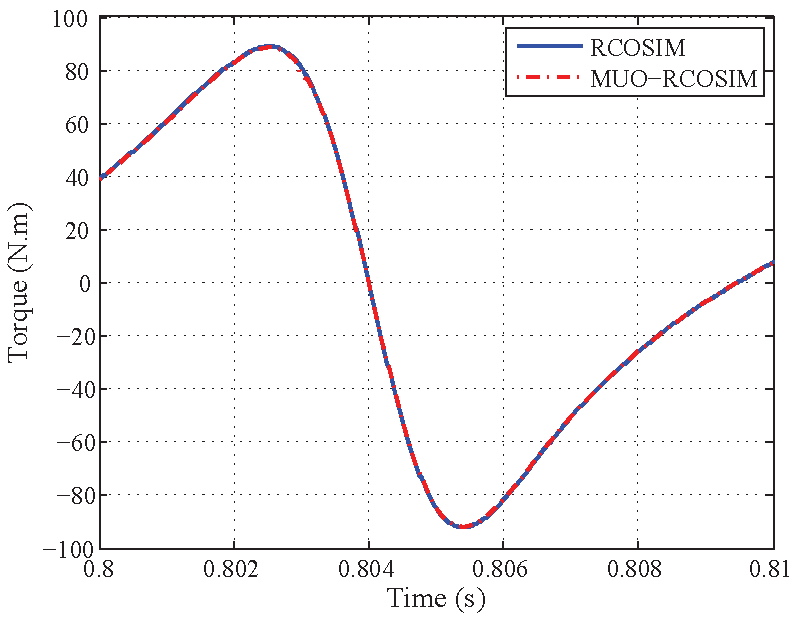
\includegraphics[scale=0.8]{figures/DF}
  \caption{Numerical results}
  \label{fig:df}
\end{figure}

\begin{figure}[htb]
\centering
  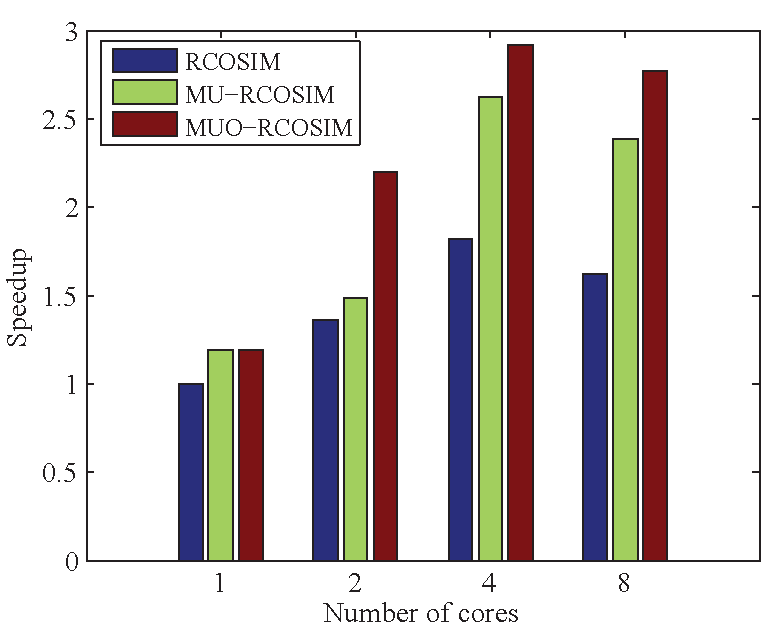
\includegraphics[scale=0.8]{figures/Speedup}
  \caption{Speedup results}
  \label{fig:spdup}
\end{figure}  

The obtained speedup and numerical accuracy results show the efficiency of our proposed method. In future work, we aim at comparing our solution with an exact scheduling algorithm and also an online scheduling approach. Also, we will test our proposed method on other industrial applications. In addition, we envision to extend MUO-RCOSIM to real-time multi-core scheduling in order to perform Hardware-in-the-Loop simulation whose main challenge is to map the real-time constraints on the different operations of the graph.